\chapter{Methodology}
\section{Kernel Selection}
So that a breadth of usage scenarios were examined, three kernels were selected based on their conformity to the following set of criteria.
\begin{itemize}
  \item \textbf{The part of the program responsible for more than two thirds of the processing time should not be more than 1500 lines.} To ensure that I fully implemented three ports of existing kernels, it was necessary to limit the size of the kernels that could be considered. This was an unfortunately necessary decision to make. Whilst it reduced the field of possible kernels, an analysis of the rejected kernels found that many of them devoted lots of code to subtle computational variations, which were of more importance to a particular rarefied domain, rather than presenting a novel approach to parallelism. (i could cite some benchmarks here like bookleaf or something)

  \item \textbf{The program must use shared memory parallelism and target the CPU.} Rust's (supposed) zero cost memory safety features are its differentiating factor. The best way to test the true cost of Rust's memory safety features would be through shared memory parallelism, where a poor implementation of memory management will make itself evident through poor performance. Programs which target the GPU rather than the CPU will not be considered, as the current implementations for Rust to target GPUs involve calling out to existing GPU APIs. Therefore, any analysis of a Rust program targeting a GPU would largely be an analysis of the GPU API itself.

  \item \textbf{The program run time should reasonably decrease as the number of threads increases, at least until the number of threads reaches 32.} It is important that any kernel considered is capable of scaling to the high core counts normally seen in HPC.I will be running the kernels on Cirrus, which supports 36 real threads.

  \item \textbf{The program operate on data greater than the CPU's L3 Cache} so that we can be sure that the kernel is representative of working on large data sets. Cirrus has an L3 cache of 45MiB. As each node has 256GB of RAM, a central constraint when working with large data sets is the speed with which data is loaded into the cache. Speed is often achieved by programs in this area through vectorisation, the use of which can be deduced from a program's assembly code. If there is a large performance difference between Rust and the reference kernels, we can use the program's assembly code to reason about that difference.

  \item \textbf{The program must be written in C or C++.} This restriction allows us to choose work which is more representative of HPC programs that actually run on HPC systems, rather than python programs which call out to pre-compiled libraries. Unlike Fortran, C and C++ use array indexing and layout conventions similar to Rust, which will make porting programs from them easier.

  \item \textbf{The program must use OMP.} This is a typical approach for shared memory parallelism in HPC. Use of a library to do the parallel processing also further standardises the candidate programs, which will lead to a deeper understanding of the kernel's performance factors.
\end{itemize}

The best kernels I found to fit this criteria were Babel Stream, sparse matrix vector multiplication and K-means clustering.

Babel Stream was developed by blah blah and it is written in C++, using OpenMP it has a good precedent of being used by blah blah, it performs operations blah blah. Tests found it to scale well so I implemented it.

\subsection{Implementation}
Implementation of all three programs follows the same process, as outlined in Figure~\ref{fig:imp-flow}. Once a candidate kernel is selected, it is implemented in Rust in serial. Any differences between the  behaviour of the Rust and the original implementation are thought of as bugs, and are eradicated or minimised as far as is possible. For ease of development, the Rust crate Clap was used to read command line arguments for the program, leading to Rust implementations of kernels being called with slightly different syntax. This difference was deemed to be superficial enough to be allowable. Kernel output was ensured to be as similar as possible to aid data-collection from both implementations.

\begin{figure}
  \center
  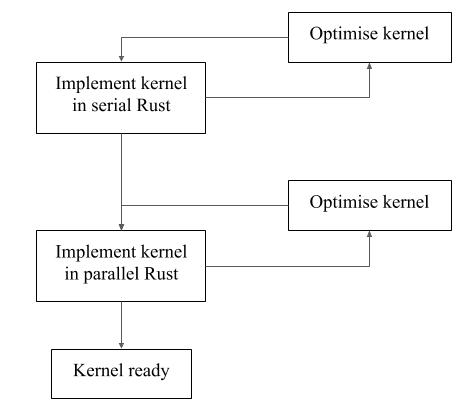
\includegraphics[height=12cm]{figs/ImplementationFlow.png}
  \caption{Flow Diagram for Implementation Process}
  \label{fig:imp-flow}
\end{figure}

Next, I would eliminate any bugs found in my serial implementation of the code by comparing outputs between my implementation and the reference implementation. During this process I would also move the code away from its C conventions towards more idiomatic Rust. To achieve more idiomatic Rust, I used the linting tool Clippy~\cite{RustClippy}, which was developed by the Rust team.  Clippy includes a category of lints under  which highlight `code that should be written in a more idiomatic way'~\cite{RustClippy}. I implemented all of Clippy's recommended rewrites, which would often include replacing the use of for loops to access vector variables with calls to the vectors \texttt{iter()} method. This particular replacement could require code to be rewritten in a much more functional style. (should I give an example?)

I would then parallelise the kernel using Rayon~\cite{RustRayon} at the same loops where the reference implementation used OpenMP to parallelise its loops. Sometimes this would be a simple matter of replacing the \texttt{iter()} method with \texttt{par_iter()}, but more parallising more complex operations like reductions and initilisations was slightly more difficult.

I would then again endeavour to fix bugs Bugs at this stage could be hard to fix as they could come from original implementations

testing is discussed in full detail next section, box could instead say `Ready for testing'

\subsubsection{Babel Stream}
\begin{itemize}
  \item Type problems due to generics leading to verbose code and obfuscating debugging
  \item The compiler did help with type debugging a little, but had limitations - give example
  \item Idiomatic serial Rust was faster than C like rust, potentially due to iter\_mut allowing optimisations? Evidence from triad and add.
  \item Once I figured out the for\_each pattern is was easy to apply it to other operations
  \item Realised that Rust's serial init was a bottleneck
  \item difficulty in writing para init as not a common use case scenario, and obfusticated by type
\end{itemize}

Initialisation is the very verbose - Explain why it's so verbose, process for finding this to be worth doing etc.
\begin{lstlisting}[language=Rust]
vec![0.0; arr_size].par_iter()
                   .map(|_| T::from(0.2).unwrap())
                   .collect_into_vec(&mut self.b);
\end{lstlisting}

Explain what's going on in this code fragment, compare it to the C original. Whilst this is a lot, Rust does reduce need for defensive coding. Could do a sloc comparison between original and new, if it was felt to be worth doing.

\begin{lstlisting}[language=Rust]
pub fn triad(&mut self){
  let scalar_imut = self.scalar;
  self.a.par_chunks_mut(self.chunk_size)
        .zip(self.c.par_chunks(self.chunk_size))
        .zip(self.b.par_chunks(self.chunk_size))
        .for_each(|((a, c), b)|
              for ((a_i, c_i,), b_i) in a.iter_mut()
                                         .zip(c.iter())
                                         .zip(b.iter()){
                                           *a_i = *b_i + scalar_imut * *c_i
                                          });
}
\end{lstlisting}

\subsubsection{Sparse Matrix}
\begin{itemize}
  \item Bit shift overflow causes Rust to crash not just run on, have to be more careful about kernel input parameters. Initially thought this might be a bug. Give example.
  \item Found init bug, was very difficult to implement para init. Filed bug report with original project
  \item remember that class you tried to build to increment stuff? m8
\end{itemize}

\subsection{Experimentation}

\section{Questionnaire}
